%% LyX 1.1 created this file.  For more info, see http://www.lyx.org/.
%% Do not edit unless you really know what you are doing.
\documentclass[english]{article}
\usepackage[T1]{fontenc}
\usepackage[latin1]{inputenc}
\usepackage{babel}
\usepackage{graphics}

\makeatletter

%%%%%%%%%%%%%%%%%%%%%%%%%%%%%% LyX specific LaTeX commands.
\providecommand{\LyX}{L\kern-.1667em\lower.25em\hbox{Y}\kern-.125emX\@}
%% Special footnote code from the package 'stblftnt.sty'
%% Author: Robin Fairbairns -- Last revised Dec 13 1996
\let\SF@@footnote\footnote
\def\footnote{\ifx\protect\@typeset@protect
    \expandafter\SF@@footnote
  \else
    \expandafter\SF@gobble@opt
  \fi
}
\expandafter\def\csname SF@gobble@opt \endcsname{\@ifnextchar[%]
  \SF@gobble@twobracket
  \@gobble
}
\edef\SF@gobble@opt{\noexpand\protect
  \expandafter\noexpand\csname SF@gobble@opt \endcsname}
\def\SF@gobble@twobracket[#1]#2{}

%%%%%%%%%%%%%%%%%%%%%%%%%%%%%% Textclass specific LaTeX commands.
 \usepackage{GECCO_proceedings2e}

\makeatother
\begin{document}

\title{An Analysis of Random Number Generators for a Hardware Implementation
of Genetic Programming using FPGAs and Handel-C}


\author{Peter Martin\\
Department of Computer Science, Essex University,\\
Wivenhoe Park, Colchester, CO4 3SQ UK}

\maketitle
\begin{abstract}
An abstract.
\end{abstract}

\section{Introduction}

Previous work \cite{martin:2001:gpem} described an implementation
of Genetic Programming using Field Programmable Arrays and a high
level language to hardware compilation system called Handel-C. Subsequent
work \cite{martin:2002:eurogp2002} described a pipelined implementation
that improved the performance and demonstrated that the technique
could be used to solve the artificial ant problem . In both cases
the work concentrated on the implementation issues and increasing
the clock speed of the implementation, but put to one side the performance
of the system with respect to it's ability to solve GP problems. Now
that the raw throughput issues have been addressed it is time to look
at how good the hardware implementation performs with respect to GP,
in particular the effectiveness of the Random Number Generator (RNG)
used. 

A comment often made about Genetic Programming and other stochastic
search methods is that a good random number generator is needed. The
evidence so far is that the quality of the RNG is probably not as
important as often stated. Nevertheless, it is important to consider
the effect of design decisions and to investigate alternatives where
practicable.

In the hardware implementation of GP, the random number generator
is implemented using a Logical Feedback Shift Register (LFSR) which
has a number of known weaknesses, which suggests that other random
number generators should be investigated. This paper begins with a
brief description of the Handel-C language and the design of a hardware
GP system. This is followed by a review of previous work on random
number generation that has been implemented in hardware. We then present
an analysis of the pseudo random number generator used in the original
design, and investigate other random number generators. We finish
with a discussion of the results and draw some conclusions.


\section{A Hardware Implementation of GP using FPGAs}

A detailed review of previous work using FPGAs in Evolutionary Computing
can be found in \cite{martin:2001:gpem}.


\subsection{Description of Handel-C}

Handel-C is a high level language that is at the heart of a hardware
compilation system known as Celoxica DK1 \cite{Celoxica:website}
which is designed to compile programs written in a C-like high level
language into synchronous hardware. The output from Handel-C is a
file that is used to create the configuration data for the FPGA. A
description of the process used by Handel-C to transform a high level
language into hardware and examples of the hardware generated can
be found in \cite{page:1996}. Handel-C has its roots in CSP and Occam.

The C-like syntax makes the tool appealing to software engineers with
little or no experience of hardware. They can quickly translate a
software algorithm into hardware, without having to learn about VHDL
or FPGAs in detail. Examples of how Handel-C may be exploited can
be found in work by Page \cite{page:video:1997} where a number of
video algorithms were implemented using just an FPGA, and in work
by Sulik \textit{et al} \cite{sulik:2000} that describes how a Reduced
Instruction Set Computer core was designed in 48 hours.

One of the advantages of using hardware is the ability to exploit
parallelism directly. Because standard C is a sequential language
Handel-C has additional constructs to support the parallelization
of code, and to allow fine control over what hardware is generated.

Since Handel-C targets hardware, there are some programming restrictions
when compared to using ISO-C, and these need to be considered when
designing code that can be compiled by Handel-C. Some of these restrictions
particularly affect the building of a GP system. Firstly, there is
no stack available, so recursive functions cannot be directly supported
by the language. Secondly, there is a severe limit to the size of
memory that can be implemented using standard logic cells on an FPGA
because implementing memory is expensive in terms of silicon real
estate. However, some FPGAs have internal RAM that can be used by
Handel-C which is supported by the \texttt{ram} storage specifier.

Handel-C supports two targets. The first is a simulator that allows
development and testing of code without the need to use any hardware.
This is supported by a debugger and other tools. The second target
is the synthesis of a netlist for input to FPGA place and route tools.
This allows the design to be translated into configuration data for
particular chips. Analysis of cycle counts is available from the simulator,
and an estimate of the final gate count is generated by the Handel-C
compiler.


\subsection{Target Hardware}

The target hardware for this work is a Celoxica RC1000 FPGA development
board fitted with a Xilinx XCV2000E Virtex-E FPGA having 43,200 logic
cells and 655,360 bits of block ram, a PCI bridge that communicates
between the RC1000 board and the host computer's PCI bus, and four
banks of Static Random Access Memory (SRAM). Logic circuits isolate
the FPGA from the SRAM, allowing both the host CPU and the FPGA to
access the SRAM, though not concurrently. 


\subsection{Program Representation}

The lack of a stack in Handel-C means that a standard tree based representation
is difficult to implement because recursion cannot be handled by the
language. An alternative to a tree representation is a linear representation
which has been used by others to solve some hard GP problems \cite{Nordin:1995:tcp}.
Using a linear representation, a program consists of a sequence of
words which are decoded by the problem specific fitness function. 


\section{Previous Work on Pseudo Random Numbers for Genetic Programming and
Hardware}

This section reviews the types of random number generators that have
been used by hardware implementations of GA, GP and other applications
of hardware to probabilistic algorithms.

Linear Feedback Shift Register (LFSR) or Tauseworth generators have
been used by Maruyama et al \cite{maruyama:19}. In their paper they
referred to the generator as a m-sequence, or maximal sequence. This
means that the generator of length \( n \) generates \( 2^{n}-1 \)
numbers. Graham \cite{Graham:96} implemented a single cycle LFSR.

An interesting hybrid was used Tommiska and Vuori \cite{tommiska:1996}
where three coupled LFSRs were used to provide a random sequence.
An interesting feature of this work is that the RNG was combined with
a source of noise. The amplified noise from a diode was fed into an
analogue to digital converter, and the resulting digital values were
used to seed the RNG, and also added to the LFSR at intervals.

The manufacturers of FPGAs provide example designs of LFSRs to be
used as random sequence generators. For example Xilinx \cite{xilinx:rng:2001},
and Altera \cite{altera:2001} provide HDL code for LFSRs.

Aporntewan \cite{aporntewan:2001} used a one dimensional 2-state
Cellular Automata (CA). Shackleford et al \cite{shackleford:2001}
implemented a CA based on the work by Wolfram \cite{Wolfram:1986}.

In the field of GP, the behavior of GP and GAs has been investigated
using different RNGs. Meysenburg and Foster considered the effect
of different RNGs on GAs \cite{meysenburg:1999:RGPR} and GP \cite{meysenburg:1999:RGQGP}.
Their conclusions were that there were no statistical differences
in the performance of GA or GP when different RNGs were used.


\section{Analysis of Random Number Generators for a Hardware GP System}


\subsection{Performance measurements}

The performance of the various RNGs in this paper was tested using
three methods. Firstly, the Diehard test suite maintained by Marsaglia
\cite{diehard:2001} was used to gauge the general performance of
the RNG. This suite consists of up to 15 tests that are modeled on
applications of random numbers. All the RNGs considered in this paper
were implemented in ISO-C and were submitted to all 15 tests. The
test method for Diehard is similar to that described in Meysenburg
and Foster \cite{meysenburg:1999:RGQGP}. Each RNG was used to generate
a binary file of about 10~MiB%
\footnote{The notation MiB indicates \( 2^{20} \) (1048576) bytes. This paper
uses the binary prefixes from the NIST.\cite{NIST:2001}
}. Each Diehard test produces one or more \( p \)-values. A \( p \)-value
can be considered good, bad, or suspect. Meysenburg used a scheme
by Johnson \cite{Johnson:1996} which assigns a score to a \( p \)-value
as follows. If \( p\geq 0.998 \) then it is classified as bad. If
\( 0.95\leq p<0.998 \) then it is classified as suspect. All other
\( p \)-values are classified as good. Every bad \( p \)-value scores
4, every suspect \( p \)-value scores 2 and good \( p \)-values
score zero. For each RNG, the scores for each test were summed, and
the total for each RNG is the sum of all the test scores for that
RNG. Using this scheme, high scores indicate a poor RNG and low scores
indicate a good RNG. The results are shown in \ref{Appendix A}.

Each RNG was then implemented using Handel-C and used in the artificial
ant problem with the Santa Fe trail. The problem was run 500 times,
and the number of correct programs that appeared was recorded. This
is used as a measure of how good the RNG performs. In all cases, the
population size is 1024, the maximum program length is 31 and all
experiments were run for 32 generations. 

Each RNG was also implemented as a stand alone application for an
FPGA using Handel-C, and the number of slices used and the maximum
attainable clock frequency was recorded. This gives a measure of the
hardware resources needed to implement the RNG, and also an indication
of the logic depth required.


\section{Random Number Generator Implementations}


\subsection{LFSR RNG}

Figure \ref{fig:LFSR} shows a schematic of the LFSR used in this
work. 


\begin{figure}[h+tb]
{\centering \resizebox*{!}{2cm}{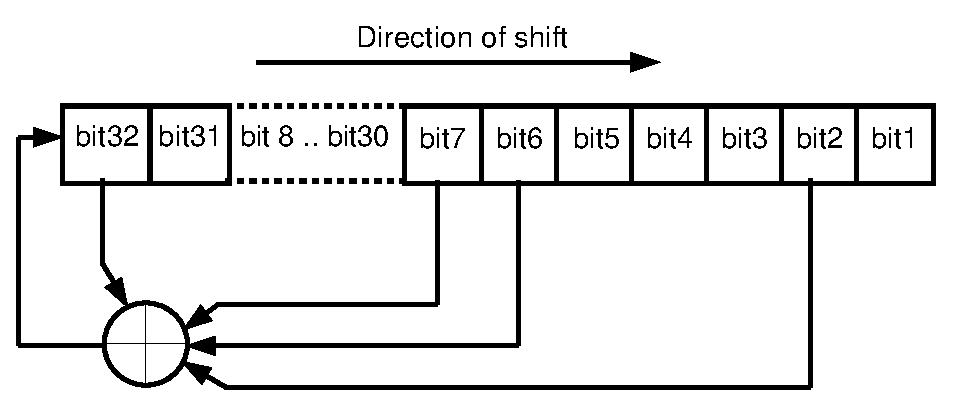
\includegraphics{images/lfsr.eps}} \par}


\caption{\label{fig:LFSR}Logical Feedback Shift Register Random Number Generator}
\end{figure}


The random number is read from the highest bits as required. The obvious
weakness of this type of RNG is that sequential values fail the serial
test described by Knuth \cite{Knuth:vol2}. At any time step \( t \)
there is a 50\% probability that the value at time \( t+1 \) can
be predicted. If for an LFSR of length \( n \) at time \( t \) the
value is \( v \), then at time \( t+1 \) the value will be \( v/2 \)
or \( v/2+2^{n-1} \). This is shown in figure \ref{fig:LFSR pairs test}
where pairs of values \( v_{t} \) and \( v_{t+1} \) are plotted. 


\begin{figure}[h+tb]
{\centering \resizebox*{!}{4cm}{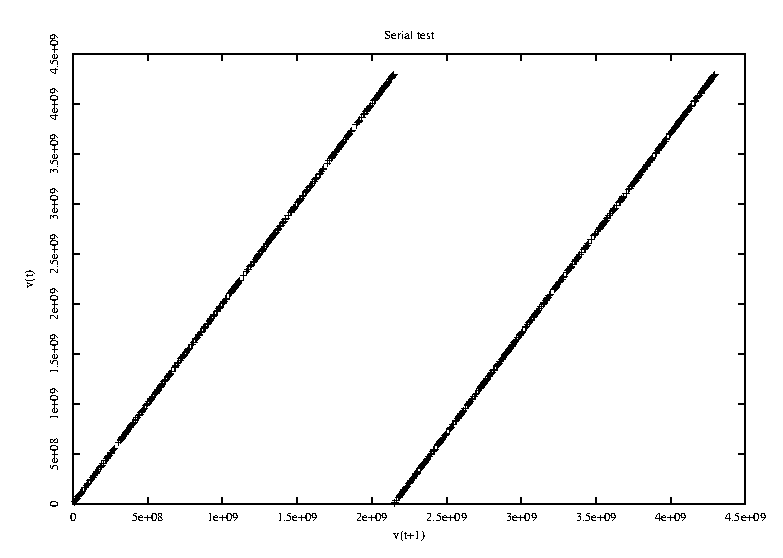
\includegraphics{images/lfsrrng_1.eps}} \par}


\caption{\label{fig:LFSR pairs test}Serial test of a simple LFSR RNG}
\end{figure}


It can be seen that for any value \( v_{t} \) there are only two
possible values of \( v_{t+1} \). Though the random number generator
runs in parallel with the main GP machine, it is possible to access
sequential values when creating an initial program, or when choosing
crossover points. There is then a possibility of a potentially degrading
bias by using such an RNG. 


\subsection{Multiple LFSRs}

One method of obtaining better serial test results for the LFSR of
length \( n \) is to allow the LFSR to run for \( n \) cycles before
reading another number. Since this would limit the rate at which random
numbers could be generated in the present design it is not explored
any further. However, an equivalent result can be obtained by implementing
\( n \) LFSRs of length \( m \) and using a single bit from each
LFSR at each time step. This can also be done using a single long
LFSR of \( n\times m \) bits, \cite{Stiliadis:1995} effectively
implementing \( n \) parallel LFSRs. However, implementing a long
shift register in a Xilinx Virtex FPGA is not efficient because the
look up tables can implement a 16 bit shift register very easily,
but longer shift registers require more extensive routing resources. 

The effect of using a better RNG was investigated by implementing
32 16 bit LFSR machines that run in parallel, and initializing each
LFSR to a different value. Bit32 from each LFSR is used to construct
a 32 bit random number. The serial test result is shown in figure
\ref{fig:16 LFSR RNG pairs test}, which shows the serial test result
for 32 LFSRs is better than the single LFSR. This generator is referred
to as the 32LFSR.


\begin{figure}[h+tb]
{\centering \resizebox*{!}{4cm}{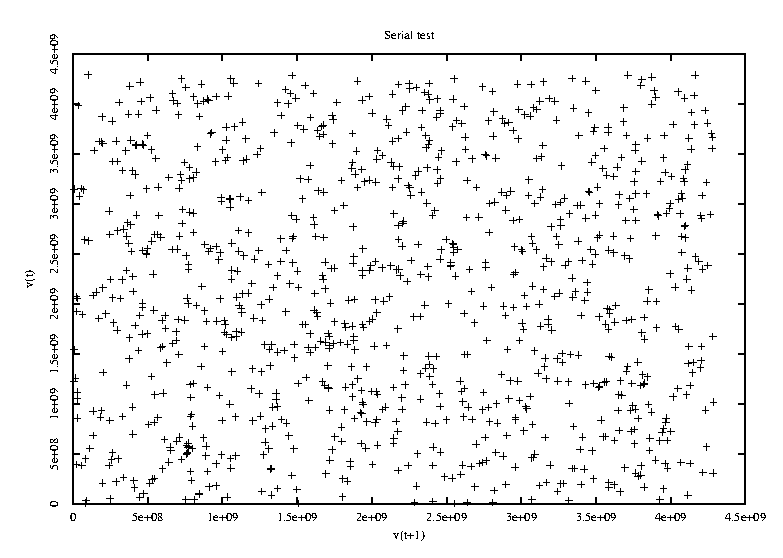
\includegraphics{images/lfsrrng_skip.eps}} \par}


\caption{\label{fig:16 LFSR RNG pairs test}Serial test for an RNG using 16
parallel LFSRs}
\end{figure}



\subsection{Cellular Automata RNG}

Another popular RNG for hardware implementations is based on Cellular
Automata (CA). A one-dimensional (1D) CA consists of a string of cells.
Each cell has two neighbors - left and right, or in some literature
west and east respectively. At each time step, the value of any cell
\( c \) is given by a rule. For this implementation, rule 30 is used,
which states that for any cell \( c \) at time \( t \), \( c_{t+1}=((west_{t} \)+\( c_{t})\oplus east_{t}) \),
where \( \oplus  \) denotes the exclusive OR function. In practice
the CA is implemented using a single 32 bit word, and for cell 0,
its right-hand neighbor is cell 31, and similarly for cell 31 its
left hand neighbor is cell 0. Figure \ref{fig:CA pairs test} shows
the result of running this RNG using the serial test. As in the simple
LFSR RNG there is a distinct pattern to the numbers, but for most
values of \( v_{t} \) there are several possible values for \( v_{t+1} \).
This generator is referred to as 1DCA.


\begin{figure}[h+tb]
{\centering \resizebox*{!}{4cm}{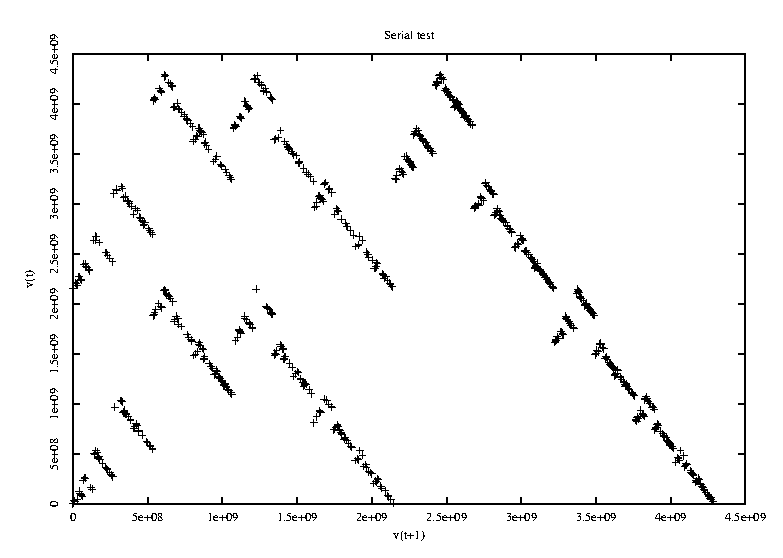
\includegraphics{images/lcarng_1.eps}} \par}


\caption{\label{fig:CA pairs test}Serial test for a 1DCA RNG}
\end{figure}



\subsection{Multiple CA generators}

As in the case of the LFSR RNG, if several CAs are combined, the results
should be much better. For this test, 32 CAs were implemented, and
by taking one bit from each CA, a 32 bit random number can be generated.
The serial test appears to be much more random, as shown in figure
\ref{fig:CA 16}. Each CA is initialized with a different pattern.
This generator is referred to as the 32CA
\begin{figure}[h+tb]
{\centering \resizebox*{!}{4cm}{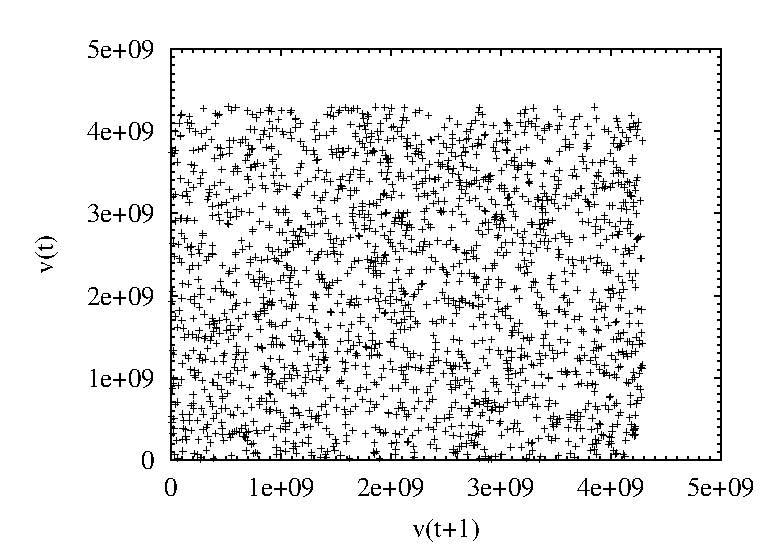
\includegraphics{images/lcarng_skip.eps}} \par}


\caption{\label{fig:CA 16}Serial test for a 32CA}
\end{figure}



\subsection{Standard C RNGs}

Another frequently used RNG is the linear congruential (LC) generator
that is often found in implementations of the standard C library.
The general equation for these is \( I_{j+1}=aI_{j}+c\mid m\mid  \),
where \( a,c \) and \( m \) are constants chosen to produce a maximal
length RNG. However, as pointed out by many authors (eg:\cite{press86numerical})
these generators are not good. Another factor against such a generator
for implementing in hardware is that it requires one addition, one
multiplication, and one modulus operator, which in Handel-C would
consume a large amount of silicon and because of the deep logic produced,
would be slow. An alternative given by \cite{press86numerical} avoids
the modulus operator, and is called the Even Quicker Generator (EQG).
It is claimed that this is about as good as any 32 bit linear congruential
generator. Its equation is \( I_{j+1}=aI_{j}+c \), and values for
\( a=1664525 \) and \( c=1013904223 \) are suggested. 

As a sanity check that the experimental method of ranking the RNGs
using Diehard was the same as that used by Meysenburg, the generator
known as ``the mother of all generators'' was also implemented and
run against the Diehard suite. This is a multiply with carry generator
and is described by Marsaglia \cite{marsaglia:1994}. It was not implemented
in the hardware GP system.


\subsection{Non random sequences}

Until now we have considered pseudo random sequences. These are sequences
where it is hard to guess the next number in a sequence. As an experiment,
a further set of runs were performed with an obviously non-number
generator. For this a sequential generator that output the sequence
\( n,n+1,n+2,\ldots  \) was used. Rather surprisingly this also worked
to produce 100\% correct programs, though substantially fewer than
the other generators achieved. 

It was only when a totally degenerate sequence of 4 numbers was tried
that GP failed to operate. This was because of the internal parallelism
in the design needs at least size unique numbers. During each generation,
a number of individual programs are being evaluated. In the test runs,
the system was configured to evaluate two programs in parallel and
at the same time two more programs are being selected using a tournament.
Programs that are being evaluated are not valid candidates for pre-tournament
selection, so we need at least six different values to be generated
by the random number generator. A small degenerate random number set
would also fail because with two functions and four terminals, there
are 64 possible instructions that can be created at initialization
time. If the degenerate set was less than 64 then not all possible
instructions can be instantiated. A small set of numbers would also
prevent individual programs being selected and possible crossover
points being ignored.


\subsection{Truly Random Sequences}

All the RNGs considered so far are not true random sequences, relying
on the manipulation of objects of finite size, and so fail one or
more of the Diehard battery of tests. So a set of random numbers was
obtained from a source generated by using the atmospheric noise captured
by a radio receiver\cite{randomorg:2002}. Each GP run for the ant
problem needs about half a million random numbers, so a block of 10~MiB
was downloaded from www.random.org, and a randomly selected 2~MiB
block was transferred to one of the SRAM on the FPGA system using
DMA. The FPGA read this block sequentially to get its random numbers.


\section{Experimental Results}

The results from running the Diehard tests are shown in the Appendix
A and are summarized in table \ref{table:Summary of Diehard}. This
shows the total results for each test and ranks them.


\begin{table}[h+tb]

\caption{\label{table:Summary of Diehard}Summary results of running the Diehard
tests on the RNGS.}

\begin{tabular}{lcc}
\hline 
RNG&
Rank&
Score\\
\hline
Mother&
1&
20\\
True&
2&
22\\
32LFSR&
3&
162\\
EQG&
4&
288\\
32CA&
5&
640\\
CA&
6&
676\\
LFSR&
7&
756\\
\end{tabular}
\end{table}


The number of correct programs that were produced by each random number
generator was recorded and is shown in table \ref{table:Correct program counts}.
The results are ranked and shows how each RNG performed. The table
also shows the slice count for the RNG implemented using Handel-C
and the maximum frequency as reported by the place and route tools.
The slice count and frequency for the true RNG assumes that the source
of random numbers is supplied by an external device to the FPGA, and
that the FPGA simply needs to read the value from a port and write
it to a register.


\begin{table}[h+tb]

\caption{\label{table:Correct program counts}Summary of GP performance for
all random number generators tested from 500 runs}

\begin{tabular}{p{1.2cm}p{0.7cm}p{1cm}p{1cm}p{0.7cm}p{1cm}}
\hline 
RNG&
Rank&
Correct&
\% Correct&
Slice&
\( F_{max} \) (MHz)\\
\hline
32CA&
1&
190&
38.0\%&
&
\\
True&
2&
188&
37.6\%&
&
\\
32LFSR&
3&
185&
37.0\%&
&
\\
EQG&
4&
182&
36.4\%&
&
\\
ID CA&
5&
182&
36.4\%&
&
\\
LFSR&
6&
159&
31.8\%&
&
\\
Sequential&
7&
59&
11.8\%&
&
\\
\hline
\end{tabular}
\end{table}



\section{Discussion}

The score obtained by the mother RNG was close to that obtained by
Meysenburg, the difference being explained by the fact that Meysenburg
used the average of 32 runs, while the work described here used only
a single run. It is probable that using 32 different seeds, that different
scores would be observed. This confirms that the experimental method
used for ranking the RNGs using Diehard is comparable.

Despite the apparently serious deficiencies found in both the simple
LFSR used in the original implementation and the simple one dimensional
CA random number generator, the overall effect of implementing a more
sophisticated RNG on the overall GP performance appeared to be small.
This result generally agrees with the work by Meysenburg and Foster
\cite{meysenburg:1999:RGPR}\cite{meysenburg:1999:RGQGP}, with the
exception that they did not consider a single-cycle LFSR. The single-cycle
performs the least well of the RNGs considered in this paper.

Even more surprising was the emergence of programs when a non-random
sequence was used. Clearly non-random sequences do not allow GP to
operate as efficiently in terms of producing 100\% correct programs,
presumably because of the failure to explore some areas of the program
space. 

Despite the small differences in performance, from the results we
can say that using a different RNG from the single LFSR would improve
the performance of the hardware GP implementation by a measurable
and therefore useful amount, and that an RNG based on multiple LFSRs
or multiple CAs would be a better choice for a hardware GP system.
The use of a truly random number source did not appear to improve
performance over the 1DCA, 32CA and 32LFSR RNGs. This provides more
evidence countering the notion that GP needs a very high quality RNG. 


\section{Further work and Conclusions}

Random numbers are used in several functions within a GP system: Initial
population creation, selection and crossover point selection. In common
with all reported GP systems, the same RNG is been used for all these
functions within a run. From a practical point of view it would appear
that there is little point is using more than one type of RNG for
different functions, but from the result using a sequence a question
arises about the role that random sequences play as opposed to sequences
that simply enumerate a set of numbers. From this it follows that
different stages in GP may use random number sequences in different
ways, and that using an enumeration may be helpful when investigating
the dynamics of GP.

The conclusion from this investigation for the hardware GP system
is that the simple LFSR used in the original design can be improved
upon by using a generator based on multiple LFSRs, multiple CAs, or
if available, a source of true random numbers. However it is clear
that the results of using a 'better' random number generator are on
the whole small.


\subsubsection*{Acknowledgments}

The author would like to thank Marconi plc for supporting this work,
Celoxica Ltd for providing access to Handel-C and Xilinx corp for
access to the place and route tools.

\bibliographystyle{plain}
\bibliography{handelc}



\section*{\newpage \label{Appendix A}Appendix A}


\subsection*{Results of the Diehard Tests}

This appendix contains the results of running the Diehard tests for
all RNGs in this paper. Max score represents the case where an RNG
fails all the tests.
\begin{table}[h+tb]

\caption{\label{table:Diehard results}Diehard test results for all RNGs considered
in this paper.}

\begin{tabular}{p{4cm}p{1cm}p{1cm}p{1cm}p{1cm}p{1cm}p{1cm}p{1cm}p{1cm}}
\hline 
Test&
Max score&
LFSR&
EQG&
32LFSR&
IDCA&
32CA&
True&
Mother\\
\hline
Birthday&
36&
36&
8&
2&
0&
8&
0&
0\\
Overlapping permutation&
8&
8&
0&
4&
8&
8&
0&
0\\
Binary Rank 32x32&
8&
8&
2&
8&
2&
6&
0&
0\\
Binary Rank 6x&
104&
104&
40&
8&
140&
70&
4&
6\\
Bitstream&
80&
80&
0&
0&
80&
80&
4&
0\\
Overlapping pairs tests&
328&
328&
188&
94&
328&
320&
6&
2\\
Count the ones (stream)&
8&
8&
8&
8&
8&
8&
0&
0\\
Count the ones (specific)&
100&
100&
42&
30&
100&
100&
2&
4\\
Parking Lot&
44&
4&
0&
0&
4&
2&
0&
0\\
Minimum Distance&
4&
4&
0&
4&
4&
4&
0&
0\\
3D spheres&
84&
4&
0&
2&
4&
2&
4&
4\\
Squeeze&
4&
4&
0&
0&
4&
4&
0&
0\\
Overlapping Sums&
44&
44&
0&
0&
6&
0&
2&
2\\
Runs&
16&
16&
0&
2&
16&
8&
0&
2\\
Craps&
8&
8&
0&
0&
8&
12&
0&
0\\
\hline
Total Passed&
876&
756&
288&
162&
676&
640&
22&
20\\
\hline
\end{tabular}
\end{table}



\end{document}
